\section{Analysis of a Gilbert cell based multiplier }

\subsection{Gilbert cell overview}
\begin{figure}[H]
	\centering
	\begin{circuitikz}
		\ctikzset{tripoles/mos style/arrows,bipoles/length=1cm}
		\ctikzset{bipoles/capacitor/height=0.5}
		\ctikzset{bipoles/capacitor/width=0.1}
		%drawing MOS
		\draw (0,0) to[Tnmos,n=M1] (0,2)
		(M1.source) node[right=3mm, above=3mm]{$M1$};
		\draw (M1.gate) to[short,-*] (-1,1);
		
		\draw (0,2) -- (-2,2)
		to[Tnmos,n=M3] (-2,4)
		(M3.source) node[right=3mm, above=3mm]{$M3$};
		
		\draw (0,2) -- (2,2) to[Tnmos,mirror,n=M4] (2,4)
		(M4.source) node[left=3mm, above=3mm]{$M4$};
		
		\draw (-2,4) -- (-3,4)
		to[Tnmos,n=M6] (-3,5.5)
		(M6.source) node[right=3mm, above=3mm]{$M6$};
		
		\draw (-2,4) -- (-1,4) to[Tnmos,mirror,n=M7] (-1,5.5)
		(M7.source) node[left=3mm, above=3mm]{$M7$};
		
		\draw (2,4) -- (1,4) to[Tnmos,n=M8] (1,5.5)
		(M8.source) node[right=3mm, above=3mm]{$M8$};
		
		\draw (2,4) -- (3,4) to[Tnmos,mirror,n=M9] (3,5.5)
		(M9.source) node[left=3mm, above=3mm]{$M9$};
		
		%drawing VLO-
		\draw (M7.gate) -- (M8.gate);
		\draw (M7.gate) -| (0,4.5);
		\draw (0,4.5) to[C=$C_{signal}$] (0,3) to[short,-*] (0,3) node[below]{$V_{LO}-$};
		
		%drawing RL and out connections
		\draw (M6.drain) -- (-3,6) to[R=$R_L$,n=RL1] (-3,7) -- (-3,7.5);
		\draw (M9.drain) --(3,6) to[R=$R_L$,n=RL2] (3,7) -- (3,7.5);
		\draw (-1,5.5) -- (3,6);
		\draw (1,5.5) -- (-3,6);
		
		%Vdd and ground
		\draw (-3,7.5) node[above=3mm,right=3cm]{$V_{dd}$} -- (3,7.5);
		\draw (M1.source) -- (0,0) node[sground]{};
		
		% VLO+-
		\draw (M6.gate) -| (-4,4.75) to[short,-*] (-4,4.75) node[left]{to $G9$};
		%-| (-4,4.7) to[short,-*] (-4,3) node[left]{to $G_9$};
		\draw (M9.gate) -| (4,4.7) to[C=$C_{signal}$] (4,3) to[short,-*] (4,3) node[below]{$V_{LO}+$};
		
		% VRF+-
		\draw (M3.gate) -| (-3,2) to[C, l_=$C_{signal}$] (-3,1) to[short,-*] (-3,0.5) node[left]{$V_{RF}+$};
		\draw (M4.gate) -| (3,2) to[C, l_=$C_{signal}$] (3,1) to[short,-*] (3,0.5) node[left]{$V_{RF}-$};
		%\draw (M4.gate) -- (3,3) to[short,-*] (3,3) node[right]{$V_{RF}-$};
		
		%Out nodes
		\draw (-3, 6) to[short,*-*] (-4, 6) node[left]{$V_{out}+$};
		\draw (3, 6) to[short,*-*] (4, 6)node[right]{$V_{out}-$};
	\end{circuitikz}
	\caption{Gilbert cell mixer}
	\label{fig:GilbetCell}
\end{figure}
A CMOS-based technology Gilbert cell based mixer is shown in figure \ref{fig:GilbetCell}, whereas the biasing network can be found in figure \ref{fig:biasNet}. This circuit exploits a differential topology to implement a double-balanced cell, providing:
\begin{itemize}
	\item Reasonable conversion gain (from one to some tens);
	\item Good input frequency components rejection at the output port, along with high linearity, thanks to the double-balanced topology;\footnote{The linearity is meant with respect to the conversion gain.}
	\item Good isolation between ports is provided by the strong suppression of spurious frequency components;
	\item Possibility of integration in CMOS technology.
\end{itemize}
\begin{figure} [H]
	\centering
	\begin{circuitikz}
		\ctikzset{tripoles/mos style/arrows,bipoles/length=1cm}
		\ctikzset{bipoles/capacitor/height=0.5}
		\ctikzset{bipoles/capacitor/width=0.1}
		%M2
		\draw (0,0) to[Tnmos,mirror,n=M2] (0,2);
		\draw (M2.source) node[left=3mm,above=3mm]{$M2$};
		\draw (M2.gate)[right] |- (M2.drain);
		\draw (M2.gate) to[short,-*] (2.5,1) node[right]{to $G_1$};
		\draw (M2.source) to[short] (0,0) node[sground]{};
		\draw (0,2) -- (-2,2) to[C=$C_{bias}$] (-2,1) node[sground]{};
		%M5
		\draw (M2.drain) to[Tnmos,mirror,n=M5] (0,4.5);
		\draw (M5.source) node[left=3mm,above=3mm]{$M5$};
		\draw (M5.gate)[right] |- (M5.drain);
		\draw (0,4) -- (-2,4) to[C=$C_{bias}$] (-2,3) node[sground]{};
		\draw (M5.gate) to[R, l_=$R_1$] (2,2.3) to[short,-*] (2.5,2.3) node[right]{to $G_3$};
		\draw (M5.gate) to[R=$R_1$] (2,3.7) to[short,-*] (2.5,3.7) node[right]{to $G_4$};
		%R2 R4
		\draw (M5.drain) to[R=$R_2$,n=R2] (0,6.3) to[R=$R_4$] (0,7.1) to[short,-*] (0,7.5) node[above]{$V_{dd}$};
		\draw (0,5.7) to[short] (0.7,5.7) to[R,l_=$R_3$] (2,5) to[short,-*] (2.5,5) node[right]{to $G_6$,$G_9$};
		\draw (0,5.7) to[short] (0.7,5.7) to[R=$R_3$] (2,6.4) to[short,-*] (2.5,6.4) node[right]{to $G_7$,$G_8$};
	\end{circuitikz}
	\caption{Biasing network}
	\label{fig:biasNet}
\end{figure}

\subsection{Gilbert cell circuit analysis}
To analyse the circuit it is necessary to give some information about the topology, how it is biased and driven. Looking at figures \ref{fig:GilbetCell} and \ref{fig:biasNet} it is possible to identify five main blocks that are described hereafter.
\paragraph{Bias net}

This net is made up of a current mirror (transistors M1 and M2, figure \ref{fig:CurrentMirror}) and the voltage reference generation network (transistor M5, R1, R2, R3, R4, R5, see figure \ref{fig:biasNet}). 

Transistor M1 of the current mirror acts as a current sink for the differential pair made up by M3 and M4, fixing the biasing current for the whole circuit. M2 sinks the current of the bias net instead.
Generally transistors which compose current mirrors are biased in the saturation region, so that their high drain impedance approximates well the behaviour of a current sink.
Being $V_{G1}=V_{GS1}$ the gate voltage of M1 we have that the transistor works in saturation if:
\begin{gather}
\label{eq:sat_m1}
V_{GS}\geq V_{th}  \\
V_{DS}>V_{od} = V_{GS}-V_{th} 
\end{gather}

\begin{figure}[H]
	\centering
		\begin{circuitikz}
		\ctikzset{tripoles/mos style/arrows,bipoles/length=1cm}
		\ctikzset{bipoles/capacitor/height=0.5}
		\ctikzset{bipoles/capacitor/width=0.1}
		%M2
		\draw (-2,0) to[Tnmos,mirror,n=M2] (-2,1.5);
		\draw (-2,3) to[I=$I_{ref}$] (M2.drain);
		\draw (M2.source) node[sground]{};
		\draw (M2.source) node[left=3mm, above=3mm]{$M2$};
		%M1
		\draw (1,0) to[Tnmos,n=M1] (1,1.5);
		\draw (M1.source) node[sground]{};
		\draw (M1.gate) -- (M2.gate) |- (M2.drain);
		%Current short
		\draw (1,3) to[short,i>=$I_0$] (M1.drain);
		\draw (M1.source) node[right=3mm, above=3mm]{$M1$};
		\draw (1.5,0) to[open, v=$V_{DS1}$] (1.5,1.5);
		\draw (M1.source) to[open,v^=$V_{GS1}$] (M1.gate);
	\end{circuitikz}
	\caption{Current mirror}
	\label{fig:CurrentMirror}
\end{figure}

The same holds for M2, which is always in saturation condition since it is diode connected (provided \ref{eq:sat_m1}). In saturation (neglecting channel modulation effects), one has that drain current only depends on the gate voltage and its expression is given by:
\begin{equation}
\label{eq:Id_quadLaw}
I_D = \mu_{n,eff} \frac{C_{ox}}{2} \frac{W}{L} (V_{GS}-V_{th})^2 = \frac{\beta_{n}}{2}V_{od}^2
\end{equation}
hence M1 keeps being in saturation till when:
\begin{equation}
V_{DS1}\geq V_{od1}= V_{th}-\sqrt{\frac{2I_0}{\beta_{n}}}
\end{equation}
therefore to have a smaller value of overdrive voltage one should have larger transistors, i.e. large W.
The output impedance is instead defined by:
\begin{equation}
 r_o = \frac{1}{\lambda I_0} \propto L
\end{equation}
where $\lambda$ models the channel modulation effect. It appears to be that longer transistors are needed to have better current sinks.
By looking at figure \ref{fig:CurrentMirror}, one finds (supposing both M2 and M1 in saturation, and $V_{GS1}=V_{GS2}=V_{DS1}=V_{DS2}$) that:
\begin{gather}
I_0 = \frac{\beta_{n1}}{2}(V_{GS1}-V_{th})^2(1+\lambda_1V_{DS1}) \notag \\
I_{REF} = \frac{\beta_{n2}}{2}(V_{GS1}-V_{th})^2(1+\lambda_1V_{GS1}) \notag
\end{gather}
hence, supposing to have equal technology parameters:
\begin{equation}
\frac{I_0}{I_{REF}} = \frac{W_1/L_1}{W_2/L_2} 
\end{equation}
Ideally the current mirroring is depending only on geometrical parameters, meaning that a very good dimension matching is required. Even if the two devices are very close to each other, within the same chip, the possibility to have variations depending on temperature does exist, i.e. $V_{th}$ and $\mu_{n,eff}$. Supposing to have equal devices with everything constant but:
\begin{gather}
K_{n1}=K_n+\Delta K_n \notag \\
V_{th,1} = V_{th}+\Delta V_{th} \notag
\end{gather}
one eventually finds that:
\begin{equation}
\frac{I_0}{I_{REF}} \simeq 1 + \frac{\Delta K_n}{K_n}+2\frac{\Delta V_{th}}{V_{od}} \notag
\end{equation}
Then, some of the possible mismatch causes are:
\begin{itemize}
	\item $K_n$, that can vary a lot in case of wide circuits;
	\item $V_{od}$ that is usually set low and varies with $V_{th}$, whose small variations can produce large differences in the two currents;
	\item difference between $V_{DS1}$ and $V_{DS2}$.
\end{itemize}
Assuming as maximum variations:
\begin{gather}
\frac{\Delta K_n}{K_n} = \pm 5 \% \notag \\
\frac{\Delta V_{th}}{V_{GS}-V_{th}} = \pm 10 \% \notag
\end{gather}
one has:
\begin{equation}
\frac{I_0}{I_{REF}} = 1 \pm 15 \% \notag
\end{equation}
A cascaded voltage divider is connected as load for M2: 
\begin{itemize}
	\item M5 is diode connected and it is used to generate the right gate bias voltage for the gain stage.
	\item A resistive voltage divider made up of R2 and R4 is used to bias the mixing stage.
	\item Resistors R1 and R3 are used to connect the bias net to the gain and mixing stages' gates. They also acts as high impedance for the RF and LO signals coming from outside the circuit and prevents them to be injected into the bias net.
	\item Capacitors C1 and C2 shunt possible non-DC disturbances coming from the Gilbert Cell, improving the bias isolation.
\end{itemize}

Noise issues will not be analysed within this treatise, even if it should be considered for a complete design. As a rule of thumb, narrow gate and low overdrive voltages should be used to lower noise contribution.(FONTE) 
Using a resistive voltage reference can be detrimental in case of voltage supply fluctuations, since a resistive voltage divider cannot reject them. However, using active devices, we would produce much more low frequency noise injection within the net.

\begin{figure}[H]
	\centering
	\begin{circuitikz}
		\ctikzset{tripoles/mos style/arrows,bipoles/length=1cm}
		%I_0 and RS
		\draw (0,0) to[short,i<=$I_0$] (0,1);
		\draw (0,1) to[R,l_=$R_S$] (-1,1) -| (-1.5,1.5) to[Tnmos,n=M3] (-1.5,2) to[twoport,l=$LO_{stage}$] (-1.5,4);
		\draw (M3.source) node[right=3mm, above=3mm]{$M3$};
		\draw (0,1) to[R,l=$R_S$] (1,1) -| (1.5,1.5) to[Tnmos,n=M4,mirror] (1.5,2) to[twoport,l=$LO_{stage}$] (1.5,4);
		\draw (M4.source) node[left=3mm, above=3mm]{$M4$};
		\draw (M3.gate) -| (-2.5,1.7) to[short,-*] (-2.5,1.75) node[below]{$V_{in1}$};
		\draw (M4.gate) -| (2.5,1.7) to[short,-*] (2.5,1.75) node[below]{$V_{in2}$};
		%Vx Vy
		\draw (M3.drain) -| (-1,2.3) to[short,-*] (-1,2.3) node[right]{$V_x$};
		\draw (M4.drain) -| (1,2.3) to[short,-*] (1,2.3) node[left]{$V_x$};
	\end{circuitikz}
	\caption{Gain stage.}
	\label{fig:GainStage}
\end{figure}

\paragraph{Gain stage}

The gain stage (shown in figure \ref{fig:GainStage}) is the linear part of the mixer. It must handle with low distortion the power coming from the input RF signal providing some amplification. The topology is suited for a low noise amplifying action(FONTE): a differential stage with source degeneration. The stage is made up of two transistors (M3 and M4) in common source configuration, biased with current by M1, and two source degeneration resistances $R_S$.

The RF differential signal modulates the current flowing into each of the two transistors, that have to be biased in saturation region. For both of them it must be ensured an wide output voltage range and a quite small overdrive voltage, along with a large drain-to-source bias voltage (required to maintain the stage in saturation during the switching of the LO stage).

To have an idea about the gain that can be obtained with this stage, one can look at the one in figure \ref{fig:GainStage}. Removing degeneration resistances one finds that the gate-to-gate mesh gives:
\begin{equation}
V_{in,1}-V_{in,2} = V_{GS3}-V_{GS4} \notag
\end{equation} 
from equation \ref{eq:Id_quadLaw}, recalling that $I_{1}+I_{2}=I_0$ and squaring:
\begin{equation}
(V_{in,1}-V_{in,2})^2 = \frac{2}{\beta_n}(I_0-2\sqrt{I_1 I_2}) \notag
\end{equation}
that once inverted yields:
\begin{equation}
I_{1}-I_{2} = \sqrt{\beta_n I_0}\cdot(V_{in,1}-V_{in,2})\cdot\sqrt{1-\frac{\beta_n}{4I_0}(V_{in,1}-V_{in,2})^2} \notag
\end{equation}
Writing the previous equation in term of $\Delta I =I_{1}-I_{2} $ and $\Delta V_{in} = V_{in,1}-V_{in,2}$ and computing the value of the slope ot this characteristic, one obtains that the \emph{maximum} differential voltage gain in equilibrium condition $\Delta V_{in} =0$ is given by:
\begin{equation}
\label{eq_statiGain}
|A_{v}|= \sqrt{\beta_{n}I_0}\cdot R_{L1}
\end{equation}
This suggest that it is better to bias the stage exactly with  $V_{GS1}=V_{GS2}$. The complete expression for equation \ref{eq_statiGain} also gives that the differential transconductance is a strongly non-linear function of the gate bias voltage. 

As we said before there it is the possibility to have mismatch between the transistors and the loads due to circuit dimensions, temperature distribution and process tolerances. Then, looking at figure \ref{fig:GainStage}, $M3 \neq M4$ and $R_1 \neq R_2$ (where input resistance of the LO stage). It can be demonstrated that the offset output voltage due to differences in the circuit parameters and dimensions is:
\begin{equation}
V_{o,offset}= \Delta V{th}+\frac{V_{GS}-V_{th}}{2}\Bigg(-\frac{\delta R}{2R}\frac{\Delta W /L}{2W/L}\Bigg) \notag
\end{equation}
To reduce this error a common centroid topology should be used in layout.
Besides, it is important to notice that R\textsubscript{L1} and R\textsubscript{L2} are both the load of a common gate stage (mixing stage of the Gilbert cell) and that the actual gain for the RF stage is a current gain. 

The small signal equivalent transconductance of the stage, once we added the source degeneration, (APPENDICE?) is given by:
\begin{equation}
\label{eq_degenGain}
G_{m,eq} = \frac{g_m}{1+g_m R_S}
\end{equation}
By adding $R_S$ we lower the RF stage's current gain, however  we also get a more linear behaviour reducing its dependency with respect to the bias point (this fact will be demonstrated later). \textbf{LINEARITA' CON OVERDRIVE?? (RAZAVI rf PAG 193)}

The two transistors have the body contact connected to ground, this means that the threshold changes accordingly to the source to body voltage, V\textsubscript{SB}:
\begin{equation}
\label{eq_thresholdV}
V_{th} = V_{th0}+\gamma_B\big(\sqrt{2\phi_P + V_{SB}}-\sqrt{2\phi_P}\big)
\end{equation}
This equation holds for all the transistors in the circuit, other than in current mirror.

\paragraph{Mixing stage}
This stage is also called \emph{switching stage}, suggesting the way we want to drive transistors M6 to M9 (figure \ref{fig:MixStage}. Also this one has a differential topology, however, not in the same way of the RF stage, we drive each pair with complementary LO signals that turn on and off cycle-by-cycle one of the two devices. A sinusoidal signal is applied to the gates (similarly one can apply a square wave), large enough to ensure the abrupt switching of the stage: when a device is on it must be in saturation (not in  triode! These are actually \emph{switch-like} transistors), while the other one must be completely interdicted.

\begin{figure} [H]
	\centering
	\begin{circuitikz}
		\ctikzset{tripoles/mos style/arrows}
		\draw (-2,4) -- (-3,4)
		to[Tnmos,n=M6] (-3,5.5)
		(M6.source) node[right=3mm, above=5mm]{$M6$};
		
		\draw (-2,4) -- (-1,4) to[Tnmos,mirror,n=M7] (-1,5.5)
		(M7.source) node[left=3mm, above=5mm]{$M7$};
		
		\draw (2,4) -- (1,4) to[Tnmos,n=M8] (1,5.5)
		(M8.source) node[right=3mm, above=5mm]{$M8$};
		
		\draw (2,4) -- (3,4) to[Tnmos,mirror,n=M9] (3,5.5)
		(M9.source) node[left=3mm, above=5mm]{$M9$};
		
		%drawing VLO-
		\draw (M7.gate) -- (M8.gate);
		\draw (M7.gate) -| (0,4.5);
		\draw (0,4.5) to[short,-*] (0,3) node[below]{$V_{LO}-$};
		
		%Out nodes
		\draw (-3, 6) to[short,*-*] (-4, 6) node[left]{$V_{out}+$};
		\draw (3, 6) to[short,*-*] (4, 6)node[right]{$V_{out}-$};
		\draw (M6.drain) to[short] (-3,7);
		\draw (M6.gate) -| (-4,3) to[short,-*] (-4,3) node[below]{$V_{LO}+$};
		\draw (M7.drain) -- (3,6);
		\draw (M8.drain) -- (-3,6);
		\draw (M9.drain) to[short] (3,7);
		\draw (M9.gate) -| (4,3) to[short,-*] (4,3) node[below]{$V_{LO}+$};
		\draw (-2,3) -- (-2,4)
		(2,3) -- (2,4);
	\end{circuitikz}
	\caption{Mixing stage}
	\label{fig:MixStage}
\end{figure}

A compromise is needed since:
\begin{itemize}
	\item small amplitude of LO signals produce slower switching speed, hence part of the power is wasted as common mode signal at the output;
	\item too large LO signals drive the MOSFET in triode region producing spikes that corrupt the output signal with unwanted feed-through  and reduces speed.
\end{itemize}
Switching speed is related to the device cut-off frequency, that for short channel devices is inversely proportional to channel length and linearly dependent to the overdrive voltage:
\begin{equation}
f_T \propto  V_{od}/L \notag
\end{equation}
suggesting that the highest overdrive and the minimum channel length should be chosen. Again, a compromise must be found among the following solutions:
\begin{itemize}
	\item Setting the available length ( the minimum is fixed by the used design kit);
	\item Selecting higher overdrive voltage one has the possibility to increase f\textsubscript{T}, however to keep our switches in saturation and to obtain a large output swing we need to keep small this quantity;
	\item Widening the gate width one has faster device, but the source to bulk capacitance increases, eventually shunting the RF signal coming from the LNA stage to ground;
	\item Reducing the current a faster commutation is achieved, along with lower transconductance though.
\end{itemize}

Even if the switching stage is not linear it is possible to define its gain and in order to do that we analyse one single pair. We recall that the gate LO signal modulates the stage drain current as a square wave, that can be written in term of its Fourier's series:
\begin{equation}
 i_D(t)=I_{pk}\Bigg(\frac{1}{2}-\frac{2}{\pi} \sum_{n=1,3,5 \dots}^{} \frac{1}{n}\sin(n\omega t)\Bigg) \notag
\end{equation} 
where only odd harmonics are present. The instantaneous gain fo the stage, related to the first harmonic is:
\begin{equation}
\label{eq_SwitchGain}
A_c|_{switch} = \frac{2}{\pi}
\end{equation}
that is neither dependent on the bias of the stage nor on the actual device transconductance.\footnote{It is however important to remember what stated above, regarding the intensity of the applied gate voltage, that further reduces this quantity in case of too large input signals. Moreover its better to notice that the stage introduces a loss rather than an actual gain.} It is important to notice that equation \ref{eq_SwitchGain} is exact in case of gate's square wave signals, whereas in case of sinusoidal driving the actual gain will be reduced because of the smoother variation of the drain current waveform.

\paragraph{Load stage} 
The load stage is formed by two resistors R\textsubscript{L} whose role is to give the stage enough gain and to set the output bias voltage through the RF drain current. They must be as matched as possible to make the differential outputs of the Gilbert cell equals.

\subsection{Mathematical analysis: conversion gain}

As already stated a mixer is a non-linear time variant system, hence a descriptive approach based on the behaviour of the cell is well suited to find the conversion gain of the cell.\footnote{It is not possible to use neither the superposition of effect nor the Laplace transform to compute the gain due to the presence of the switching pairs.} 
The following analysis is based on the schematic in figure \ref{fig:GCmath}.

We suppose all the transistors in the gain and bias stage working in saturation, then we identify:
\begin{itemize}
	\item i\textsubscript{3} and i\textsubscript{4} the current through M3 and M4;
	\item i\textsubscript{6} and i\textsubscript{7} the current through M6 and M7;
	\item i\textsubscript{8} and i\textsubscript{9} the current through M8 and M9;
	\item i\textsubscript{o1} the current through R\textsubscript{L1};
	\item i\textsubscript{o2} the current through R\textsubscript{L2};
	
	\begin{figure}[H]
		\centering
		\begin{circuitikz}
			\ctikzset{tripoles/mos style/arrows,bipoles/length=1cm}
			\ctikzset{bipoles/capacitor/height=0.5}
			\ctikzset{bipoles/capacitor/width=0.1}
			%drawing MOS
			\draw (0,0) to[Tnmos,n=M1] (0,1.6) to[short,i<=$I_0$] (0,1.7) -- (0,2)
			(M1.source) node[right=3mm, above=3mm]{$M1$};
			\draw (M1.gate) -| (-1,0.8) to[short,-*] (-1,0.8);
			
			\draw (0,2) -- (-2,2)
			to[Tnmos,n=M3] (-2,3.3) to[short,i<=$i_3$] (-2,4)
			(M3.source) node[right=3mm, above=3mm]{$M3$};
			
			\draw (0,2) -- (2,2) 
			to[Tnmos,mirror,n=M4] (2,3.3) to[short,i<=$i_4$] (2,4)
			(M4.source) node[left=3mm, above=3mm]{$M4$};
			
			\draw (-2,4) -- (-3,4)
			to[Tnmos,n=M6] (-3,5.5)
			(M6.source) node[right=3mm, above=3mm]{$M6$};
			
			\draw (-2,4) -- (-1,4) to[Tnmos,mirror,n=M7] (-1,5.5)
			(M7.source) node[left=3mm, above=3mm]{$M7$};
			
			\draw (2,4) -- (1,4) to[Tnmos,n=M8] (1,5.5)
			(M8.source) node[right=3mm, above=3mm]{$M8$};
			
			\draw (2,4) -- (3,4) to[Tnmos,mirror,n=M9] (3,5.5)
			(M9.source) node[left=3mm, above=3mm]{$M9$};
			
			%drawing VLO-
			\draw (M7.gate) -- (M8.gate);
			\draw (M7.gate) -| (0,4.5);
			\draw (0,4.5) to[C=$C_{signal}$] (0,3) to[short,-*] (0,3) node[below]{$v_{LO}-$};
			
			%drawing RL and out connections
			\draw (M6.drain) to[short,i<=$i_6$] (-3,6) to[short,i^<=$i_{01}$] (-3,6.8) to[short] (-3,7) to[R=$R_L$,n=RL1] (-3,8) -- (-3,8.3);
			\draw (M7.drain) to[short,i<=$i_7$] (-1,5.8) to[short,i<=$i_{02}$] (-1,6.8) to[short] (-1,7)to[R,l_=$R_L$,n=RL2] (-1,8) -- (-1,8.3);
			\draw (-1,6) to[short,i>=$i_9$] (1,5.75) -- (3,5.5);
			\draw (-3,6) to[short,i_>=$i_8$](-1,5.75) -- (1,5.5);
			
			%VO diff
			\draw (-1,6.8) to[short,-o] (-1.3,6.8);
			\draw (-3,6.8) to[short,-o] (-2.7,6.8);
			\draw (-1.3,6.8) to[open,v=$v_{od}$] (-2.6,6.8);
			%Vdd and ground
			\draw (-3,8.3) node[above=2mm,right=6mm]{$V_{dd}$} -- (-1,8.3);
			\draw (M1.source) -- (0,0) node[sground]{};
			
			% VLO+-
			\draw (M6.gate) -| (-4,4.75) to[short,-*] (-4,4.75) node[left]{to $G9$};
			%-| (-4,4.7) to[short,-*] (-4,3) node[left]{to $G_9$};
			\draw (M9.gate) -| (4,4.7) to[C=$C_{signal}$] (4,3) to[short,-*] (4,3) node[below]{$v_{LO}+$};
			
			% VRF+-
			\draw (M3.gate) -| (-3,2) to[C, l_=$C_{signal}$] (-3,1) to[short,-*] (-3,0.5) node[left]{$v_{RF}+$};
			\draw (M4.gate) -| (3,2) to[C, l_=$C_{signal}$] (3,1) to[short,-*] (3,0.5) node[left]{$v_{RF}-$};
			%\draw (M4.gate) -- (3,3) to[short,-*] (3,3) node[right]{$V_{RF}-$};
			
			%Out nodes
			%\draw (-3, 6) to[short,*-*] (-4, 6) node[left]{$V_{out}+$};
			%\draw (-1, 6) to[short,*-*] (0, 6)node[right]{$V_{out}-$};
		\end{circuitikz}
		\caption{Gilbert cell, to be use as a reference for the mathematical analysis}
		\label{fig:GCmath}
	\end{figure}
	
	\item I\textsubscript{D} the bias current, equal to $\frac{I_0}{2}$;
	\item i\textsubscript{od} the output differential bias current;
	\item $S(t)=\frac{1}{2}-\frac{2}{\pi} \sum_{n=1,3,5 \dots}^{} \frac{1}{n}\sin(n\omega_{LO} t)$ is the switching function of the mixing cell (then we consider the LO stage as it was made up of ideal switches).
\end{itemize}
The differential input RF signal is given by:
\begin{equation}
\label{eq_inRFSignal}
v_{RF}(t)=\frac{V_{RF}}{2}\cos (\omega_{RF}t) 
\end{equation}
Currents flowing into the two RF stages are given by:
\begin{align}
i_3(t) &= I_D + i_d(t)\\
i_4(t) &= I_D - i_d(t)
\end{align}
where, from equation \ref{eq_degenGain}, the $i_d$ current is a small signal variation given by:
\begin{align}
i_d(t)&=I_{RF}\cos (\omega_{RF}t) \notag \\
&= G_{m3,4}\frac{V_{RF}}{2}\cos (\omega_{RF}t) 
\end{align}
It is now possible to define the current flowing into the switching stage recalling that they are discontinuous functions modulated by the switching function S(t):
\begin{align}
 i_6(t) &= [I_D + i_d(t)]S(t) \\
 i_7(t) &= [I_D + i_d(t)]S(t-T_{LO}/2)
\end{align}
and 
\begin{align}
i_8(t) &= [I_D - i_d(t)]S(t-T_{LO}/2) \\
i_9(t) &= [I_D - i_d(t)]S(t)
\end{align}
because M6 and M9 share the same LO signal; the same holds for M7 and M8. 
Hence the current through R\textsubscript{L1} and R\textsubscript{L2} is given by:
\begin{align}
i_{o1}(t) &= I_6(t)+I_8(t) \notag \\
&=[I_D + i_d(t)]S(t)+[I_D - i_d(t)]S(t-T_{LO}/2) 
\end{align}
and 
\begin{align}
i_{o2}(t) &= I_7(t)+I_9(t) \notag \\
&=[I_D + i_d(t)]S(t-T_{LO}/2)+[I_D - i_d(t)]S(t) 
\end{align}
Therefore, the output differential current is:
\begin{align}
\label{eq_Iod1}
i_{od}(t) &= i_{o1}(t)-i_{o2}(t) \notag \\
&=2i_d(t) S(t)-2i_d(t)S(t-T_{LO}/2) 
\end{align}
Noticing that:
\begin{align}
\label{eq_SwitchingEquality}
S(t-T_{LO}/2) &=\frac{1}{2}-\frac{2}{\pi} \sum_{n=1,3,5 \dots}^{} \frac{1}{n}\sin(n\omega_{LO} t-T_{LO}/2) \notag \\
&= \frac{1}{2}+\frac{2}{\pi} \sum_{n=1,3,5 \dots}^{} \frac{1}{n}\sin(n\omega_{LO} t) \notag \\
& =1- \frac{1}{2}+\frac{2}{\pi} \sum_{n=1,3,5 \dots}^{} \frac{1}{n}\sin(n\omega_{LO} t) \notag \\
&= 1 - S(t)
\end{align}
\begin{figure}[H]
	\centering
	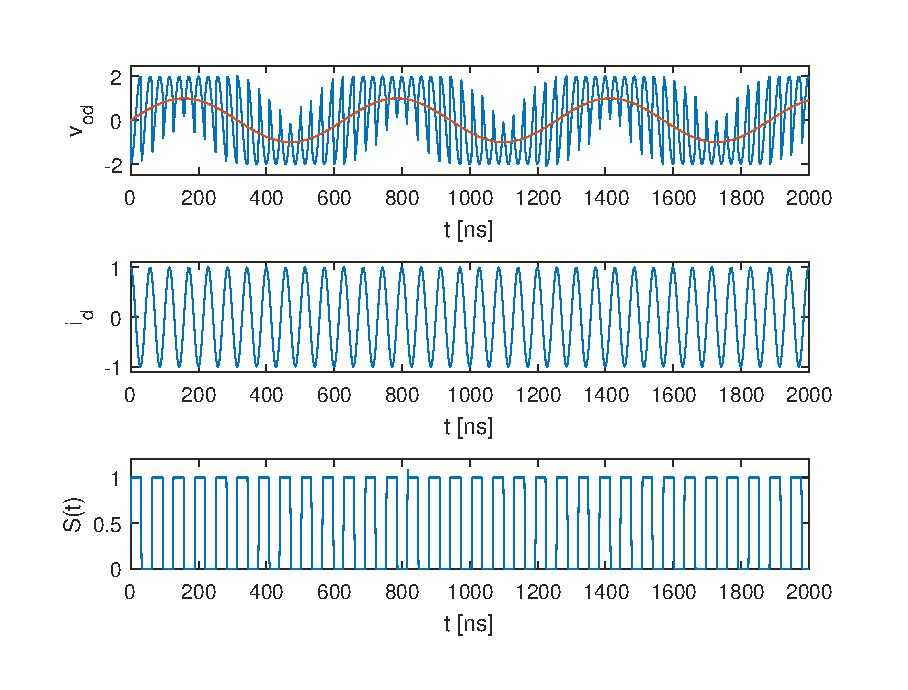
\includegraphics[scale=0.6]{ideal_WF}
	\caption{Ideal signal modulation within Gilbert cell.}
	\label{ideal_WF}
\end{figure}
and substituting equation \ref{eq_SwitchingEquality} in \ref{eq_Iod1} we get:\footnote{$cos(x)sin(y)=\frac{1}{2}sin(x+y)+\frac{1}{2}sin(x-y)$}
\begin{align}
\label{eq_Iod2}
i_{od}(t) &= -\frac{8i_d(t)}{\pi}\sum_{n=1,3,5 \dots}^{} \frac{1}{n}\sin(n\omega_{LO} t) \notag \\
&= -\frac{8I_{RF}}{\pi}\cos(\omega_{RF}t)\sum_{n=1,3,5 \dots}^{} \frac{1}{n}\sin(n\omega_{LO} t) \notag \\
&= -\frac{8I_{RF}}{\pi}\sum_{n=1,3,5 \dots}^{} \frac{1}{n}\cos(\omega_{RF}t)\sin(n\omega_{LO} t) \notag \\
&= -\frac{8I_{RF}}{\pi}\sum_{n=1,3,5 \dots}^{} \frac{1}{2n}\Big\{ \sin[(\omega_{RF}+n\omega_{LO})t]+\sin[(\omega_{RF}-n\omega_{LO}) t]\Big\}
\end{align}
The full ideal output differential signal is shown in figure \ref{ideal_WF}. Considering only the fundamental tone of the LO signal (other frequency terms are out-of-band with respect to IF) and multiplying by $R_L=R_{L1}=R_{L2}$ one finds that the differential output voltage is given by:
\begin{align}
v_{od}(t)& = -\frac{4I_{RF}R_L}{\pi}\{\sin[(\omega_{RF}+\omega_{LO}) t]+\sin[(\omega_{RF}-\omega_{LO}) t]\} \notag \\
& = -\frac{4I_{RF}R_L}{\pi}[\sin(\omega_{HF} t)+\sin(\omega_{IF} t)]
\end{align}
then, referring to the IF component:
\begin{align}
v_{od,IF}(t)& = -\frac{4I_{RF}R_L}{\pi}\sin(\omega_{IF} t) \notag \\
& = -\frac{2G_{m3,4}R_LV_{RF}}{\pi}\sin(\omega_{IF} t) 
\end{align}
that, considering the IF and RF \emph{rms} values eventually yields the Gilbert cell mixer conversion gain:
\begin{equation}
\label{eq:ConvGain}
A_{vC} = \frac{2}{\pi}\frac{R_L}{\frac{1}{g_{m3,4}}+R_S}
\end{equation}
It is now possible to highlight that:
\begin{itemize}
	\item in first approximation the conversion gain does not depends on the amplitude of the LO signal;
	\item both LO and RF components are rejected at the output;
	\item it is possible to keep only the IF component by filter out the HF signal;
	\item the degeneration resistance R\textsubscript{S} improve the stage's linearity. In fact, if properly chosen, one has: $A_{vC}|_{g_m3,4 \ll R_S}\simeq\frac{2}{\pi}\frac{R_L}{R_S}$. Besides to linearity, the conversion gain is less sensitive with respect to the RF stage bias point;
	\item no informations about frequency behaviour appear with this kind of analysis.
\end{itemize}  


